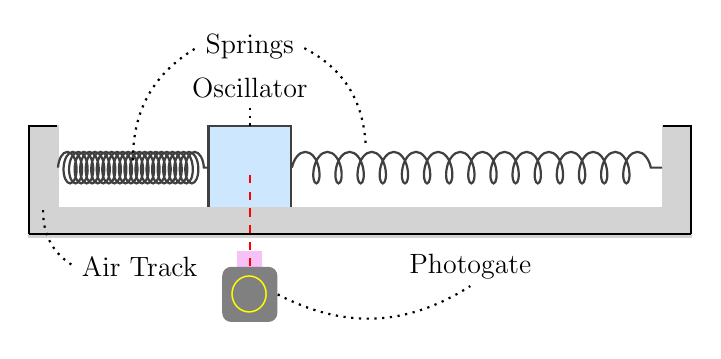
\begin{tikzpicture}[scale=0.7, transform shape]

\tikzstyle{M1}=[rectangle,draw=none,fill=darkgray!60,minimum size=1.5cm]
\tikzstyle{spring}=[darkgray,thick,decorate,decoration={aspect=0.5, segment length=4, amplitude=2mm,coil}]
\tikzstyle{ground}=[fill=LightGray,draw=LightGray,very thick]

\begin{scope}
% \node[M1,yshift=2cm,xshift=5.25cm,fill=yellow,rotate=20](p4x){};
\node[M1,yshift=-1.95cm,xshift=-2cm,minimum size=0.5cm,fill=Violet!50,draw=white,thick](p4x){};
\node[M1,yshift=-2.5cm,xshift=-2cm,fill=gray, rounded corners=0.75ex,minimum size=1cm,text=Yellow!100](p4x){\huge$\bigcirc$};
% \node[M1,yshift=2cm,xshift=5.25cm,minimum size=.7cm,rounded corners=4ex,rotate=18,text=white](p5x){};
\node[M1,yshift=-0.2cm,xshift=-2cm,fill=DodgerBlue!22,draw=darkgray,thick](p3x){};
% \node[M1,fill=none,xshift=7.45cm,yshift=-1cm,minimum size=1.25cm](m2){};
\node[ground,minimum width=12cm,minimum height=0.5cm,yshift=-1.2cm](p1x){};
\draw[thick] (-6,-1.4) -- (6,-1.4);
% \node[] at (0,2cm) {\Large Equilibrium Position};
\node[ground,minimum width=0.5cm,minimum height=1.5cm,xshift=-5.75cm,yshift=-0.2cm](LWall){};
\draw[thick] (-6,-1.4) -- (-6,0.55) -- (-5.5,0.55);
\node[ground,minimum width=0.5cm,minimum height=1.5cm,xshift=5.75cm,yshift=-0.2cm](RWall){};
\draw[thick] (6,-1.4) -- (6,0.55) -- (5.5,0.55);
\draw [spring, segment length=2] (LWall.east) -- (p3x.west)  node[midway, above](p2x1){};
\draw[spring, segment length=8] (p3x.east) -- (RWall.west)  node[midway, above](p2x2){};
\end{scope}

\begin{scope}[yshift=1.5cm]
        \node [xshift=-4cm, yshift=-3.5cm, anchor=center] (p1) {\Large Air Track};
        \node [xshift=-2cm, yshift=0.5cm, anchor=center] (p2) {\Large Springs};
        \node [xshift=-2cm, yshift=-0.25cm, anchor=center] (p3) {\Large Oscillator};
        \node [xshift=2cm, yshift=-3.5cm, anchor=center] (p4) {\Large Photogate};
        % \node [anchor=east] (p5) {\Large Spring's Restoring force};
  \end{scope}

% \begin{scope}[yshift=-9.5cm]
% \draw[gray,yshift=-6cm] (0,2.3) -- coordinate (x axis mid) (6,2.3);
% \foreach \x in {0,...,6}
%      		\draw[yshift=-6cm,gray,text=red] (\x,2.8) -- (\x,2.3)
% 			node[anchor=north] {\x};
% \foreach \xx in {1,...,60}
%             \draw[yshift=-6cm,gray] (\xx/10,2.6) -- (\xx/10,2.3){};

% \draw[<->,thick,yshift=-6cm] (0,3) -- node[above] {\huge $x$} ++(2,0);
% \draw[lightgray,very thick, dashed] (2,0.8)--(7,0.8){};
% \draw[->,lightgray,very thick, dashed,yshift=-10pt,xshift=10pt] (7.15,0.8)--(7.15,-2.1){};
% \filldraw [fill=gray,yshift=-10pt] (7.15,0.8) circle (10pt) node (pul) {};

% \node[M1,yshift=-0.2cm,xshift=2cm,fill=orange!40](m1){};
% \node[M1,text=lightgray!30,xshift=7.45cm,yshift=-3.1cm,minimum size=1.25cm](m2){\huge $\bm m$};
% \node[rectangle,rounded corners=0.4ex,draw=none,fill=blue!50,minimum size=0.32cm,yshift=0.7cm,xshift=2cm](p1x){};
% \node[ground,minimum width=12cm,minimum height=0.5cm,yshift=-1.2cm,text=white](atrackb){};
% \node[] at (0,-2) {\huge Displacement $x$, caused by force = $mg$};
% \node[ground,minimum width=0.5cm,minimum height=1.5cm,xshift=-5.75cm,yshift=-0.2cm](LWallb){};
% \node[ground,minimum width=0.5cm,minimum height=1.5cm,xshift=5.75cm,yshift=-0.2cm](RWallb){};
% \draw[line width=2mm, line cap=round, lightgray, opacity=0.5] (7.15,1.5) -- (pul.north);
% \draw [spring,segment length=8] (LWallb.east) -- (m1.west) node[midway, above](s1){};
% \draw[spring, segment length=2](m1.east) -- (RWallb.west) node[midway, above](s2){};
% \end{scope}

        \path[thick] (LWall.south) edge [dotted, bend right] (p1.west);
        \path[thick] (p2x1.center) edge [dotted, bend left] (p2.west);
        \path[thick] (0.1,.25cm) edge [dotted,bend right] (p2.east);
        \path[thick] (p3x.north) edge [dotted] (p3.south);
        \path[thick] (p4x.east) edge [dotted,bend right] (p4.south);
        \path[thick, red] (p4x) edge [dashed] (p3x.center);

\end{tikzpicture}